\documentclass{article}
\usepackage[utf8]{inputenc}
\usepackage[T1]{fontenc}
\usepackage{natbib}
\usepackage{graphicx}
\usepackage[french]{babel}
\usepackage{glossaries}

\title{GPGPU - Project report}
\author{Nicolas Portal - Alexandre Yvart - Geoffrey Jount}


\begin{document}
\pagenumbering{gobble}
\maketitle


\pagebreak
\tableofcontents


\pagebreak
\pagenumbering{arabic}

\section{Introduction}

For educational purpose in the GPGPU subject, we are asked to work on a project
using a GPU parallel method. We will use the CUDA library.

\section{Problem description}

This project's goal is to implement an image segmentation algorithm :
the max-flow/min-cut algorithm. A picture containing numerous pixels however,
processing one after another in a simple \texttt{for} loop would show to be
very slow. We thus need to make the process parallel, and implement it on GPU
for an even faster result : the \textit{push-relabel} algorithm, parallel
version of the first mentioned, is what we seek.

\section{CPU implementation}

We followed the guidelines found on the NVIDIA presentation.\\
All in all there are eight matrices :\\
- for the heights of each node\\
- for the excess flow of each node\\
- for the links between the source and each node\\
- for the links between the sink and each nodes\\
And the four last matrices for the links between each nodes : top, bottom, right and left neighbours matrices were labeled with the inverse of the euclidean distance in RGB space.\\
The links between the source and each node and the links between the sink and each node were labelled with the inverse of the average distance to the marked pixels in RGB space. Each node were linked to the source and sink. The height of each node was 0 except for the source which had a height equals to the number of nodes. The \texttt{std\string_load} library was used to load \texttt{jpg} images both in grayscale and RGB color space. Images were stored as one dimensional vectors with contiguous red, green and blue pixels. the size of these vectors were three times as large as the number of pixels in an image. The \texttt{ppm} file format was used to generate the output segmented image.

\subsection{Issue 1}

Our implementation soon ran into an infinite loop which remained one of the core issue for several weeks. As a result, the code was changed to make it possible for each node to push towards the sink or the source. This did not solved the issue. The weights of links between the source ans sink on one hand and every node on the other hand was changed using the histogram on red, green and blue channel of the marked pixels to compute a probability. This did not solved the issue as well.\\
\\
It was found that there was actually no infinite loop but the algorithm was very long to terminate as two nodes would often exchange flow between them waiting for one of them to reach the maximum height. To solve this glitch, it was decided to manually lower the maximum height. The maximum height was no longer set to the number of nodes but rather to a low number such as five or ten. This made it possible for our algorithm to terminate.

\begin{center}
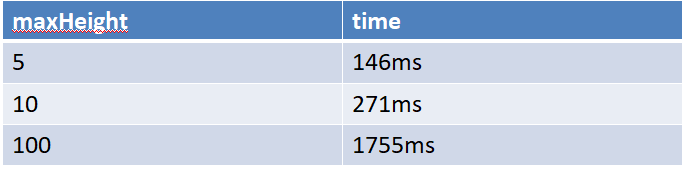
\includegraphics[scale=0.6]{pics/maxHeight benchmark.PNG} 
\end{center}

\subsection{Issue 2}

An other issue quickly appeared. Using a depth first search to find nodes yielded bad results as every pixel would be set to white.\\
\\
When it comes to the way to get the output image, it was decided to set every pixel with a height above zero to one. This did not generate optimal results but it was good enough to make out the segmentation.\\
\\
A small eight by eight image was used to make the debug step simpler. This image was a ppm image with every pixels on the top part of the image set to blue and every pixel on the lower part of the image set to red. One pixel was set to black and white in each region.

\subsection{Issue 3}

Although the maximum height was decrease to five or ten, the run time was still to high. It took 15 to 20 minutes for the algorithm to terminate.\\
\\
Lowering the maximum height resulted in a 15, 20 minute running time. This was still too high. It was found out that calling the push and relabel function on every nodes would decrease the run time significantly. The check for active nodes was now done by the push and relabel function. It was no longer needed to write a separate function to retrieve the right active nodes. It was also no longer required to loop on every pixels to find active nodes. This decreased the run time to 10 seconds which was a huge improvement.

\subsection{Issue 4}

For a long time we simply checked the height value of each pixel to get the min cut of the graph and thus decide the color of each pixel.\\
\\
Since we were not satisfied with our output segmented image, it was decided to change the way we recovered the min cut. Although there were very little explanation about the way the BFS algorithm should have been implemented in NVIDIA slides, the algorithm was successfully implemented. It was a little bit of a disapointment though since this did not change the look of the output segmented image. This led us to understand that this non optimal segmented image resulted from a flaw in the core algorithm (maybe the weights of the links).

\section{optimization}

It was found out that the count active function slowed down the algorithm. \\
\\
In order to make it quicker, It was decided to no longer loop on the whole excess flow matrix but rather, to return true as soon as the function found an active node. This slight change required to change the return type of the function from int to bool. It was not necessary to count every active nodes anymore. The program would keep in the main while loop as long as the count active function returned true. This resulted in a slight but noticeable decrease in run time.

\begin{center}
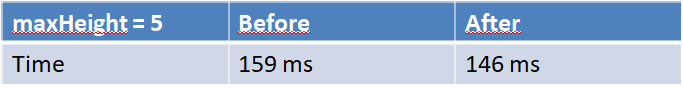
\includegraphics[scale=0.6]{pics/countactive.PNG} 
\end{center}

\section{Output segmented images}

\begin{center}
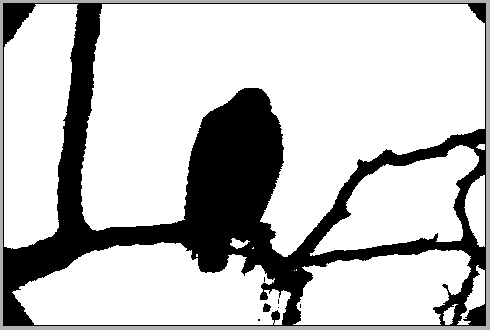
\includegraphics[scale=0.6]{pics/eagle_segmented.PNG} 
\end{center}

\begin{center}
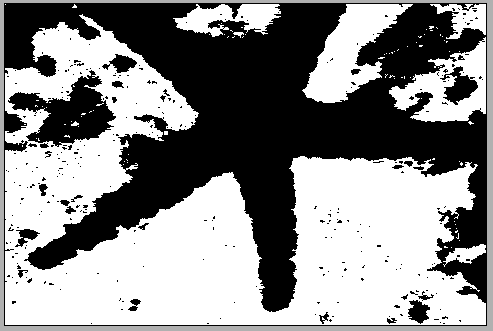
\includegraphics[scale=0.6]{pics/height 5.PNG} 
\end{center}

\begin{center}
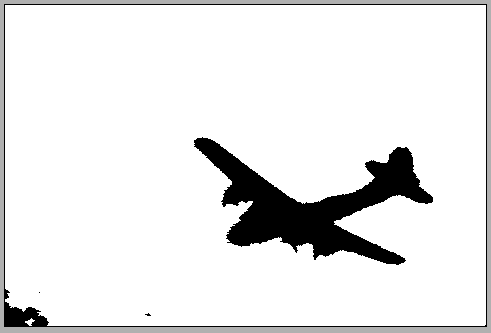
\includegraphics[scale=0.6]{pics/plane segmented.PNG} 
\end{center}

\begin{center}
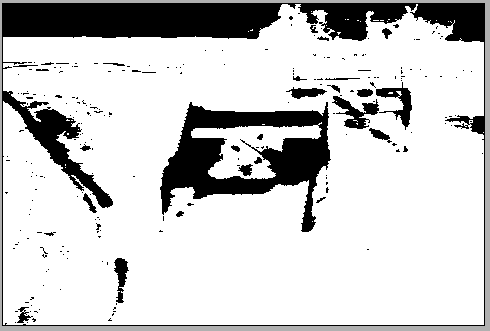
\includegraphics[scale=0.6]{pics/racing car segmented.PNG} 
\end{center}

\section{GPU implementation}
The first GPU implementation is kept as close as possible to the CPU version. The graph structure is instantiated on the CPU just like the CPU version, except that we flattened the matrices on one dimension. The graph structure is then copied on the device, with the addition of a swap matrix used for the relabeling step. Then, the push and relabel kernels are called one after the other, where each thread is representing one node of the graph. The final cut is done just like the CPU version. We didn't have much issues on implementing the GPU version since the CPU version was already functional.

\begin{center}
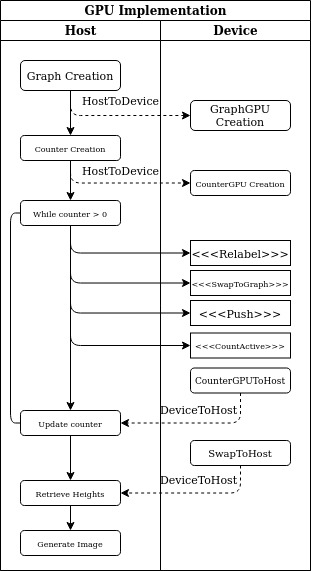
\includegraphics[scale=0.6]{pics/gpu_diagram.jpg}
\end{center}

\section{Bottlenecks}
After proceeding to some profiling, we quickly saw that our kernel used to count\_active nodes was a bottleneck because it was taking too much time despite not doing any calculus. Otherwise,  most of the bottlenecks are on the allocation of memory on the device which is hard to optimize unless by allocation the whole structure at once. The push kernel is also a bottleneck since it's checking a lot of conditions. Overall, except from reducing the number of calls to cudaMalloc, we can only solve the bottlenecks with algorithmic optimizations.

\begin{center}
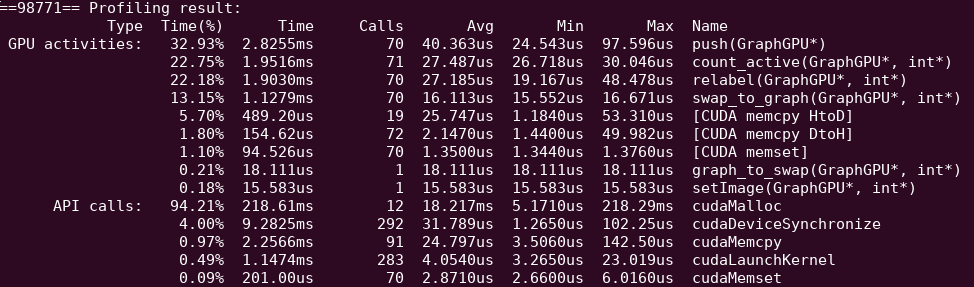
\includegraphics[scale=0.5]{pics/gpu_prof1_cut.png}
\end{center}

\section{Enhancements}

\subsection{Enhancement 1}
We reduced the time spent on the count\_active kernel by removing the atomic operations. We didn't need to count how many nodes were active but instead we just had to check if none were active. So, by using a boolean we allowed concurrent accesses to the variable and reduced the time spent on counting nodes by half.

\begin{center}
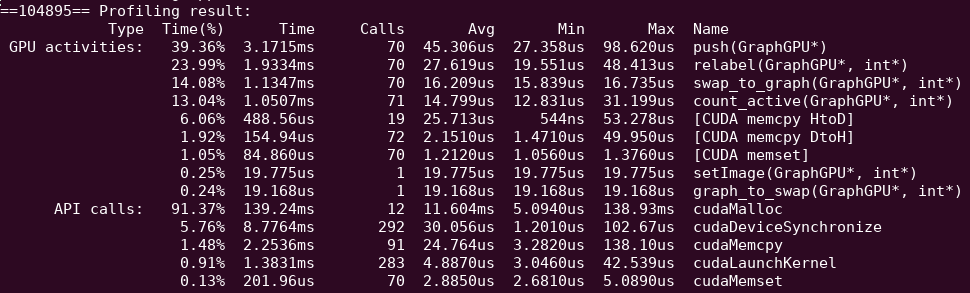
\includegraphics[scale=0.5]{pics/gpu_prof2_cut.png}
\end{center}
\newpage

\subsection{Enhancement 2}
Since most of the time spent by the API calls is on cudaMalloc, we reduced the number of allocation by 1 to gain 10 ms of execution time.

\begin{center}
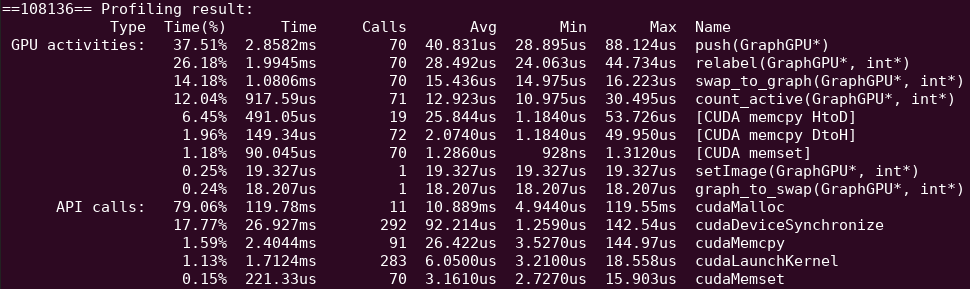
\includegraphics[scale=0.5]{pics/gpu_prof3_cut.png}
\end{center}

\section{Benchmarks recapitulation}

\begin{center}
    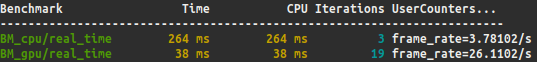
\includegraphics[width=1\textwidth]{pics/benchmark02.png}
\end{center}


\section{Tasks repartition}

\noindent
Nicolas\\
- CPU implementation and debug\\
- Report\\
- GPU debug\\
\\
Alexandre\\
- CPU debug\\
- GPU implementation\\
\\
Geoffrey\\
- CPU debug\\
- Benchmarking implementation
\end{document}
